\section{Mitbewerber Modell}
\label{sec:Mitbewerber}
Die grundlegende Idee des Konzeptes: Mitbewerber Modell ist es, die Daten von der Konkurrenz zu benutzen um daraufhin Preisvorschläge zu generieren. 
\newline
\newline
Durch dritt Anbieter wie \emph{HQ-Revenue} können Konkurrenzdaten genutzt werden um ein Modell aufzubauen. HQ-Revenue ist ein Anbieter, welcher Internetseiten wie Bookings.com oder trivago \emph{scraped} um an Hotelpreise oder andere Daten zu kommen. Dabei gibt es viele verschiedene Vorgehensweisen um Preise für ein Hotel ohne Vergangenheitsdaten zu entwickeln. Ein Primitiver Ansatz dabei wäre es, wenn alle Preise von den Konkurrenten genommen werden und damit der Durchschnitt ermittelt wird. Dies hat natürlich nichts mit Maschine Learning oder geschweige denn Data Science zu tun aber es wäre ein Ansatz der Verfolgt werden könnte. 
\newline
\newline
Dieser Ansatz birgt jedoch eine Problematik: Nicht jeder Kunde von happyhotel hat auch automatisch Konkurrenzdaten zur Verfügung, diese müssen noch dazu gebucht werden. Deswegen wird folgender Ansatz verfolgt. 
\newline
\newline
So wie im vorherigen Konzept \emph{\nameref{sec:all_Hotels}} werden auch hier die Hotels in eine Vergleichbare Form gebracht. Das Ziel ist es dann ein oder mehrere Hotels zu finden, die vermeintlich ähnlich sind. Sobald ein oder mehrere ähnliche Hotels gefunden worden sind, können die Konkurrenzdaten von den ähnlichen Hotels genutzt werden. 
\newline
\newline
Als Zielvariable des Modells werden dann die Preise des ähnlichsten Hotels verwenden.  Jedoch sollen hierbei die Preise von den Konkurrenten und von dem ähnlichsten Hotel nicht einfach so benutzt werden, sondern lediglich das Verhältnis. Die Preise sollen anhand von dem Durchschnittlichen Preis in Verhältnis gebracht werden und dieses Verhältnis soll vorhergesagt werden. 
\newline
\newline 
Das Hotel ohne Vergangenheitsdaten muss in diesem Fall dann einen Durchschnittlichen Preise angeben, anhand dessen mit dem vorhergesagten  Verhältnis der tatsächliche Preis abgeleitet werden kann. Dies soll im folgenden Schaubild noch einmal dargestellt werden:
\begin{figure}[h]
    \centering
    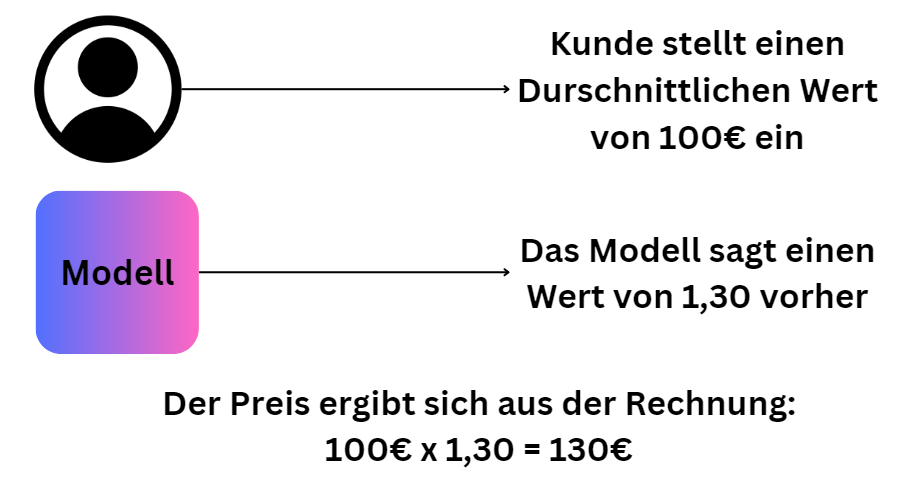
\includegraphics[width=0.5\textwidth, center]{Mitbewerber_model.png}
    \caption[Mitbewerber Modell]{Mitbewerber Modell}
    \label{img:all_hotels}
\end{figure}
